\documentclass[letterpaper, 10 pt, conference]{ieeeconf}  % Comment this line out if you need a4paper
\IEEEoverridecommandlockouts
 
\usepackage{cite}
% \usepackage{natbib}
\usepackage{amsmath,amssymb,amsfonts}
% \usepackage{algorithmic}
\usepackage{graphicx}
\usepackage{textcomp}
%%%%%%%%%%%%%%%%new package%%%%%%%%%%%
\usepackage{color}
\usepackage{subfigure}
\usepackage{multirow}
\usepackage{multicol}
\usepackage{makecell}
\usepackage{bm}
\usepackage{algorithm}
\usepackage{algpseudocode}
\usepackage{hyperref}
%%%%%%%%%%%%%%new command%%%%%%%%%%%%%
\newcommand{\ie}{i.e.\ }
\newcommand{\eg}{e.g.\ }
\newcommand{\Reffig}[1]{Figure~\ref{#1}}
\newcommand{\Refsec}[1]{Section~\ref{#1}}
\newcommand{\Refalg}[1]{Algorithm~\ref{#1}}
\newcommand{\Refeq}[1]{Equation~\eqref{#1}}
\newcommand{\Reftab}[1]{Table~\ref{#1}}
\newcommand{\COMMENT}[1]{\textcolor{red}{ (#1) }}
\newcommand{\REVISE}[1]{\textcolor{blue}{ (#1) }}
\newcommand{\HK}[1]{\textcolor{green}{ (#1) }}
\newcommand{\BLOCK}[1]{\fbox{\parbox{\textwidth}{#1}}}
\hypersetup{hidelinks,
        colorlinks=true,
        allcolors=blue,
        pdfstartview=Fit,
        breaklinks=true}
\usepackage{graphics} % for pdf, bitmapped graphics files
\usepackage{epsfig} % for postscript graphics files
\usepackage{algorithm}
\usepackage{algpseudocode}
\usepackage{amsmath}
\usepackage{amssymb}
\usepackage{subfigure}
\usepackage{graphicx}
\usepackage{subfigure}
\usepackage{booktabs}
\usepackage{threeparttable}
\usepackage{multirow}
\usepackage{multicol}
\usepackage{makecell}
\usepackage{dcolumn}
\usepackage[T1]{fontenc}
\usepackage{diagbox}

%%%%%%%%%%%%%%%%%%%%%%%%%%%%%%%%%%%%%
\begin{document}
\title{
        LOG-LIO: A LiDAR-Inertial Odometry with Efficient Local Geometric Information Estimation
}

\author{Kai Huang$^{1}$, Junqiao Zhao$^{*,2, 3}$, Tiantian Feng$^{1}$, Zhongyang Zhu$^{3}$, Chen Ye$^{2}$% <-this % stops a space
        \thanks{$^{1}$Kai Huang and Tiantian Feng are with the School of Surveying and Geo-Informatics, Tongji University, Shanghai, China
                        {\tt\footnotesize (e-mail: huangkai@tongji.edu.cn; fengtiantian@tongji.edu.cn).}}
        % \thanks{This work is supported by the National Key Research and Development Program of China (No. 2021YFB2501104) \COMMENT{john: verify before submission}. \emph{(Corresponding Author: Junqiao Zhao.)}}% <-this % stops a space
        \thanks{This work is supported by the National Key Research and Development Program of China (No. 2021YFB2501104). \emph{(Corresponding Author: Junqiao Zhao.)}}% <-this % stops a space
        \thanks{$^{2}$Junqiao Zhao, Zhongyang Zhu and Chen Ye are with Department of Computer Science and Technology,
                School of Electronics and Information Engineering, Tongji University, Shanghai, China, and the MOE Key Lab of Embedded System and Service Computing, Tongji University, Shanghai, China
                        {\tt\footnotesize (Corresponding Author: zhaojunqiao@tongji.edu.cn; 1930773@tongji.edu.cn; yechen@tongji.edu.cn).}}
        \thanks{$^{3}$Institute of Intelligent Vehicles, Tongji University, Shanghai, China}
}

\maketitle

\begin{abstract}

        Local geometric information, \ie{normal and point distribution}, is crucial for LiDAR-based simultaneous localization and mapping (SLAM) because it provides constrains for data association, which further determines the direction of optimization and ultimately affects the accuracy of poses.
        However, estimating normal and point distribution are time-consuming tasks even with the assistance of the KDtree or volumetic maps.
        To achieve fast normal estimation, we look into the structural information of LiDAR scan and propose a novel fast approximate least squares (FALS) method.
        With the pre-computed bearing information, estimating the normal requires only the range information of the points when a new scan arrives.
        To efficiently estimate the distribution of points, we extend the ikd-tree to manage the map in voxels and update its point cloud distribution incrementally while maintaining its consistency with the normals.
        For scan points that satisfy visibility and consistency checks based on normal, we devise a robust and accurate hierarchical data association schema considering the distribution where point-to-surfel is prioritized over point-to-plane.
        We further fix voxels after the distribution convergences to balance the time consumption and the correctness of representation.
        Extensive experiments on diverse public datasets demonstrate the advantages of our system compared to other state-of-the-art methods.
        % Our open source implementation is available at \href{https://github.com/tiev-tongji/LOG-LIO}{https://github.com/tiev-tongji/LOG-LIO}.
\end{abstract}

% \titlepgskip=-15pt

\section{INTRODUCTION}
\label{sec:introduction} % labels should always start with a prefix  sec:, fig: tab:
% \COMMENT{use present tense throughout the paper}

% \COMMENT{The introduction should first explain the role of normal in LIO (background) and then why is it crucial to propose an efficient normal estimation method for LIO (motivation). The motivation can be explained based on the point-to-surfel metric and incremental map updates}

% \COMMENT{a paper should only focus on a few key issues.}

Simultaneous localization and mapping (SLAM) plays an important role in autonomous driving and robotics tasks.
% Compared with visual-inertial systems \cite{qin2018vins, geneva2020openvins, campos2021orb}, 
LiDAR(-inertial) systems \cite{shan2020lio, ye2019tightly, qin2020lins, reinke2022locus2} are robust and accurate because they are less sensitive to illumination changes and have a larger field of view (FoV).

% The accuracy of LiDAR-based system depends on point cloud registration, which associates similar geometric features between two point clouds, and minimizes the distance between them.
The accuracy of LiDAR-based system depends on the registration between point cloud and map, which associates them according to the similarity of local geometric information and then minimizes their distances.
Therefore, accurate and fast estimation of local geometric information has gained increasing attention in recent studies \cite{chen2022direct, nguyen2023slict, reinke2022locus2, palieri2020locus, ramezani2022wildcat}.
Normal and point distribution are two representative local geometric properties of the surface where a point is located, but estimating any one of them is a time-consuming task for LiDAR-inertial odometry (LIO) systems even with the assistance of the KDtree or volumetic maps.
Therefore the previous LIO systems seldom incorporate the real-time estimation of normal and point distribution, which may undermine the real-time performance of the systems.

The conventional method for estimating local geometric information is to evaluate the smoothness of the input scan points and fit the features to the map points, respectively \cite{zhang2014loam}.
Further, optimization minimizes the distance from the point to the corresponding feature along the normal direction, which also depends on the local geometric information.
However, simple smoothness calculations do not take into account information about adjacent scan lines, and the coordinates of map points do not accurately represent the spatial distribution of neighbors, which may degrade the accuracy of the LIO system.
Estimating local geometric information efficiently in the LIO system remains a challenge.

% \COMMENT{The review of specific normal estimation method should be put in the related work.}
% Normal estimation of point cloud has been well studied in recent decades.
% \cite{rusu20113d} build a KDtree with point cloud to search the adjacent area of the point, and then fit the plane to estimate the normal.
% However, considering LiDAR point cloud is disordered, it will consume a lot of time when building KDtree and searching, which cannot meet the real-time requirements of LiDAR SLAM systems.
% It should be noted that, like data association module of LOAM\cite{zhang2014loam}, adjacent information can be quickly and simply established from adjacent scan lines based on point indexes.
% But the point cloud indexes of different scan lines are also disordered in most LiDARs, that is, the nearest point cannot be directly obtained according to the indexes of points.
% Therefore, searching for the nearest point on the adjacent scan lines is similar to KDtree and still needs to traverse every point on the adjacent scan line, which is also time-consuming.
% Inspired by \cite{badino2011fast} and \cite{fan2021three}, we look into the structural information of LiDAR scan lines(rings), and propose a novel fast least-squares approximation(Ring FALS) based on this instead of using a KDtree to search the K-NN neighborhood.
This paper presents LOG-LIO, a robust and accurate LIO system focusing on the estimation of local geometric information, including efficiently estimating the normal of LiDAR scanning points and the distribution of map points, and their rational utilization.

Inspired by \cite{badino2011fast} and \cite{fan2021three}, we look into the structural information of LiDAR scan and propose a novel fast approximate least squares (FALS) method.
% With the pre-computed bearing directions information, estimating the normal requires only the range information of the points when a new scan arrives.
We project point cloud onto the range image to pre-build a lookup table, which stores the bearing information for the certain LiDAR.
With the arrival of a new scan, only the range of the point is needed to estimate the normal, and the matrix inversion operation is not performed in the calculation, which greatly improves the efficiency.
% Because the scanning line (ring) plays an important role in our method, we name it Ring FALS.
% To facilitate the community, we open source the Ring FALS normal estimator as an independent tool, which is available at \href{https://github.com/tiev-tongji/RingFalsNormal}{https://github.com/tiev-tongji/RingFalsNormal}.

We incrementally update the point cloud distribution within the map voxels to keep the correctness of the spatial information while maintaining its consistency with the normals.
To balance time consumption and correctness of representation, we manage the map on the extended ikdtree and further fix the distribution after it converges.

% Similar to the FAST-LIO series \cite{xu2021fast, xu2022fast}, we do not perform feature extraction on raw points, but directly associate point cloud with voxels on the map after distortion correction.
% % Like FAST-LIO series, we do not perform feature extraction on point cloud, but instead directly associate the point cloud with map voxels after undistortion.
% For scan points that satisfy visibility and consistency checks based on normals, we devise a robust and accurate hierarchical data association schema considering the distribution, where large-scale point-to-surfel associations have the highest priority.
% % We design a data association scheme where point-to-surfel is preferred over point-to-plane, and large-scale is prioritized over small-scale.
% % Similar to SLICT\cite{nguyen2023slict}, by analyzing the spatial information of the nearest map voxels, small-scale distribution are simply merged into large-scale distribution.
% The pose is optimized by integrating the IMU measurements as initial estimates and then using an error-state iterative Kalman filter \cite{xu2021fast} to minimize the multi-scale point-to-surfel and point-to-plane distances.

The main contributions of this work are listed as follows:
\begin{itemize}
        \item
              Ring FALS, a novel fast approximate least squares normal estimator using the structural information of certain LiDAR, is fast and accurate compared to PCL, and meets the real-time requirements of the LIO system.
        \item
              A robust and accurate hierarchical data association schema considering the distribution of points within map voxels where point-to-surfel is prioritized over point-to-plane and large-scale over small-scale.
              %       We incrementally update the distribution of points inside map voxels managed by the extended ikd-tree, while maintaining the consistency with the normals.
        \item
              Extensive experiments on public datasets demonstrate the advantages of our LIO system compared to other state-of-the-art methods.
              To benefit the community, our implementation of this work is open-source at \href{https://github.com/tiev-tongji/LOG-LIO}{https://github.com/tiev-tongji/LOG-LIO}, and we also open-source Ring FALS as an independent normal tool at \href{https://github.com/tiev-tongji/RingFalsNormal}{https://github.com/tiev-tongji/RingFalsNormal}.
\end{itemize}

% We abbreviated this work to LOG-LIO for short.
% The rest of the paper is structured as follows:
% %todo
% In Sect. \ref{sec:related_work}, we discuss relevant literature.
% Ring FALS normal estimation and map voxels distribution incrementally update are detailed in Sect. \ref{sec:ring_fals} and Sect. \ref{sec:distribution_surfel}, respectively.
% An overview of the complete system pipeline is given in Sect. \ref{sec:system_overview}.
% The data association and map management are presented in Sect. \ref{sec:data_association} and \ref{sec:map_management} respectively.
% implementation details and experimental results are shown in Sect. \ref{sec:experimental_results}.
% Finally, the paper is concluded with a discussion and possible future research direction in Sect. \ref{sec:conclusion_and_future_work}.

\section[sec:related_work]{RELATED WORKS} % another way of labeling a section
\label{sec:related_work}

\subsection{Point Cloud Normal Estimation}

% Since LiDAR acquire a set of point samples on real surfaces, the normal at a certain point on surfaces can be computed in two ways\cite{rusu2010semantic}:
% first, reconstruct the spatial topological relationship of the acquired point cloud dataset, using surface meshing techniques, and then compute the surface normals from mesh;
% second, approximately inferring surface normals directly from point cloud datasets.
% For the real-time performance of LiDAR-based SLAM, computational power is a limited resource and it is difficult to build the topological relationship of the point cloud in advance.
% The above limitations prevent us from meshing the point cloud to compute the normals in SLAM.

The most common method to obtain surface normals form point cloud is the least squares due to its relatively low computational cost and ease of implementation\cite{rusu20113d}.
% However, least squares becomes computational expensive when applied to LiDAR point cloud, which have thousands of measurements per millisecond.
% Not to mention that because of the disorder of LiDAR point cloud, it is usually necessary to build a KDtree to search the neighborhood of every point, which is also a time-consuming step.
However, even without considering the disorderly nature of LiDAR point cloud, the least squares method is computationally expensive for LIO systems.
% \cite{badino2011fast} compared the complexity of least squares approaches, including traditional total least squares, normalized least squares, unconstrained least squares and fast approximate least squares(FALS).
\cite{badino2011fast} compares the complexity of least squares approaches, and by reformulating the traditional least squares solution, the normal can be estimated by calculating the derivatives of surface from a spherical range image (SRI).
However, with a large $k$ neighborhood, usually $k$ greater than 5 is more reliable, the time consumption of SRI is greater than FALS.
3F2N\cite{fan2021three} simply performs three filtering operations on the inverse depth image to estimate the normals, which is slightly faster than FALS, and the accuracy is strongly influenced by the filter.
However, 3F2N is designed for RGBD camera point cloud and requires neighborhood information of pixels, making it not directly applicable to LiDAR point cloud.

Inspired by \cite{badino2011fast} and \cite{fan2021three}, we propose Ring FALS, a normal estimator for LiDAR point cloud.
By analyzing the spatial geometric information of the disordered LiDAR point cloud, we pre-compute and store its structural information in a lookup table.

\subsection{Points Distribution Estimation}
LOAM \cite{zhang2014loam} does not estimate the distribution of points, but performs eigen analysis on the associated map points to determine whether its local geometry is close to a line or a plane.
However, the coordinates of a few neighborhood points cannot accurately represent local geometric information, which results in providing inaccurate constraints.

% DLO\cite{chen2022direct} is a direct method with a lightweight front end that without feature extraction or distortion correction.
Different from the LOAM point-to-line and point-to-plane ICP algorithm, DLO\cite{chen2022direct} registers point cloud using Generalized ICP (GICP)\cite{segal2009generalized} to minimize the plane-to-plane distances,
and these planes are modeled by the computed covariance of each point in the scan.
It assumes that the submap covariances can be approximated by concatenating the normals from keyframes and the covariance of the points is only computed once when the scan is acquired.
However, such a stitching normals method cannot accurately represent the local geometric information of the point cloud, which ultimately affects accuracy.

LOCUS 2.0\cite{reinke2022locus2} extends the work of LOCUS\cite{palieri2020locus}, which constructs custom covariance matrices based on the pre-computed normals for GICP, but how to pre-compute normals is not elaborated in their paper.

Wildcat\cite{ramezani2022wildcat} generate surfels by clustering points based on their coordinates and timestamps, and then fits ellipsoids to them based on the distribution of point coordinates.
% It employed a multi-resolution scheme where the clustering and surfel extraction steps are repeated at multiple spatial resolution.
Similar to Wildcat, SLICT\cite{nguyen2023slict} proposes an octree-based global map and incrementally updates the point distribution within voxels incrementally.
It obtains large-scale distribution by merging multiple voxels.
Inspired by the above, we extend ikd-tree to maintain the positions and update points distribution of map nodes incrementally.
We manage map nodes in the extended ikd-tree with voxels, and then fix the voxel to surfel after its distribution convergences.

\subsection{LiDAR(-Inertial) Odometry}

LOAM\cite{zhang2014loam} has inspired many LiDAR SLAM systems due to the relative independence of the system modules and the rationality of using point cloud geometry attributes.
% The LiDAR SLAM process it designed can be devided into feature extraction, odometry and mapping.
% Feature extraction, odometry and mapping are the three modules designed by LOAM.
% In feature extraction, it divided point cloud into edge and plane features according to the smoothness of adjacent points on the same scan line.
% The odometry module perform high-frequency scan-to-scan point cloud registration using iterative closest point(ICP) algorithm\cite{besl1992method} on different features to estimate the LiDAR odometry in real-time.
% With the odometry, the mapping module perform low-frequency scan-to-map point cloud registration to refine the LiDAR pose on the map.
% Inertial Measurement Unit(IMU) is optional for correcting distortion of point cloud.
However, the lack of effective map management and the huge optimization time consumption can reduce the performance of the system.
% LeGO-LOAM\cite{shan2018lego} proposes a lightweight framework that estimates real-time 6 degree-of-freedom pose for ground vehicles.
% It segments ground point cloud and performs feature extraction to obtain distinctive planar and edge features.
% LeGO-LOAM\cite{shan2018lego} segments ground point cloud to speed up computation and uses a two-step Levenberg-Marquardt optimization method to solve different components of the six degree-of-freedom transformation.
% But the ground point cloud segmentation is only applicable to horizontally placed LiDARs.
% LeGO-LOAM reduces long-term drift with a loop closure module, but the ground point cloud segmentation is only applicable to horizontally placed LiDARs.

% In the LiDAR-Inertial SLAM systems, the IMU is used to correct the distortion of point cloud and provide an initial value for the registration of point cloud and map.
% Compared with LiDAR SLAM systems, the LIO systems are more robust with IMU high-frequency acceleration and angular velocity measurements.
LIO-SAM proposes a framework based on keyframes and local maps, which optimizes poses in a factor graph\cite{kaess2012isam2}.
However, LIO-SAM builds sub-maps for input scans by simply merging point cloud of surrounding keyframes, which is a time-consuming construction when the number of points is large.
FAST-LIO\cite{xu2021fast} adopts the error-state iterated extended Kalman filter(iEKF) to directly register the undistortion point cloud and map.
It presents a new formula to compute the Kalman gain and the computation load depends on the state dimension.
FAST-LIO2\cite{xu2022fast} maintains the map by an incremental KDtree data structure, namely ikd-tree, to further improve efficiency.
In this paper, we adopt the iEKF as FAST-LIO to optimize poses by directly registering point cloud and map, but with a different data association schemas.
By incorporating normal and points distribution, we construct surfel and associate with it in priority, since surfel is more representative of the local geometric properties of a small region.

\section{PRELIMINARY}
\label{sec:preliminary}

\subsection{Notation}
\label{sec:notation}
We now define notions and frame definitions that we used throughout the paper.
We consider $\mathcal{W} $ as the world frame and ${\mathcal{I} _k}$, ${\mathcal{L} _k}$ as the IMU and LiDAR frames, related to the $k$-th LiDAR scan at time $t_k$, respectively.
$^a\mathbf{T}_b \in SE(3)$ to be Euclidean transformation take 3D points from frame $b$ to frame $a$, which consisted of rotation $^a\mathbf{R}_b \in SO(3)$  and translation $^a\mathbf{t}_b \in \mathbb{R}^3$.

\subsection{LiDAR Observation Model}
\label{sec:lidar_obser}
\begin{figure}[!ht]
        \centering
        \subfigure[LiDAR observation model]
        {
                \begin{minipage}[b]{0.2\textwidth}
                        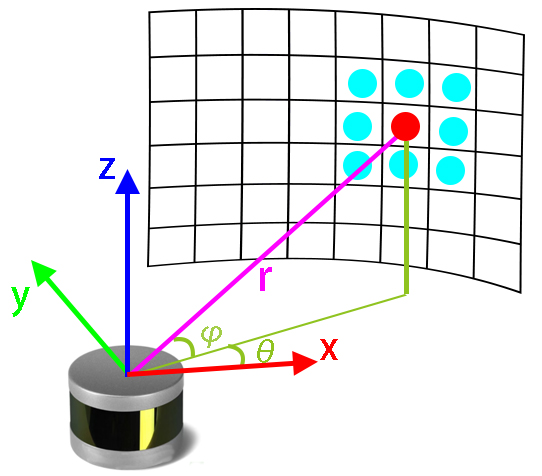
\includegraphics[width=1\textwidth]{fig/lidar_obser.jpg}
                \end{minipage}
                \label{fig_lidar_obser}

        }
        \subfigure[ point distribution merged]
        {
                \begin{minipage}[b]{0.2\textwidth}
                        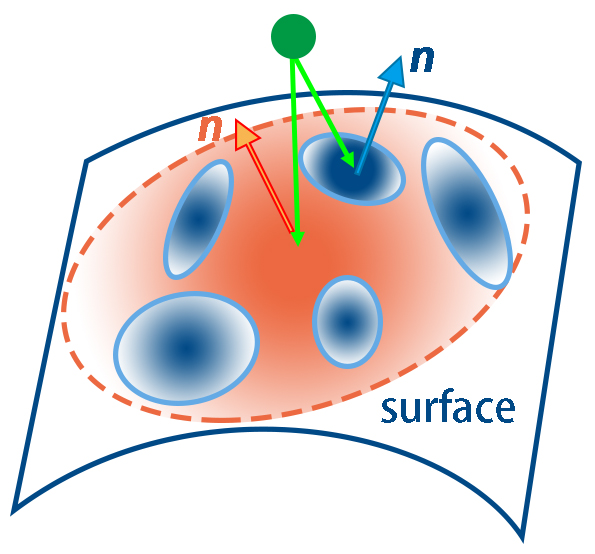
\includegraphics[width=1\textwidth]{fig/data_association_2.jpg}
                \end{minipage}
                \label{fig_association}
        }
        \caption{Illustration of the LiDAR observation model and point distribution merged.
                (a) The magenta line indicates the range of the red point.
                The 8 cyan points are the neighborhoods that Ring FALS uses to estimate the normal of the target point.
                (b) The 5 blue ellipses represent the nearest neighbors of the green query point in the extended ikd-tree,
                and are merged into the large-scale orange distribution.
        }
\end{figure}
% \begin{figure}[!ht]
%         \centering
%         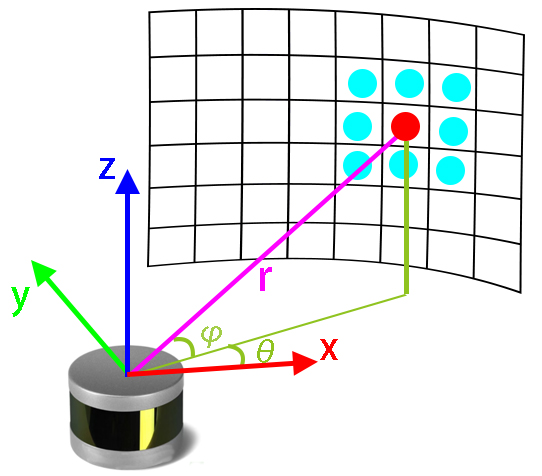
\includegraphics[width=3.5 cm]{fig/lidar_obser.jpg}
%         \caption{Illustration of the bearing and the range of a target point.
%                 The red point is the target that the LiDAR is measuring, and the magenta line indicates the range.
%                 The 8 cyan points are the neighborhoods that Ring FALS uses to estimate the normal of the target point.}
%         \label{fig_lidar_obser}
% \end{figure}
In practice, LiDAR obtains the 3D coordinates of a point by combining bearing and range measurements of the target surface\cite{yuan2021pixel, yuan2022efficient}, as shown in Fig. \ref{fig_lidar_obser}.
% The transformation between them is as follows:
The LiDAR observation model is as follows:
\begin{equation}
        \boldsymbol{p}_i = r_i\boldsymbol{v}_i = r_i \left[\begin{array}{c}
                        \cos \theta_i \cos \varphi_i \\
                        \sin \theta_i \cos \varphi_i \\
                        \sin \varphi_i
                \end{array}\right]
        \label{eq_p_rv}
\end{equation}
where $r_i$ is the range, $\theta_i$ the azimuth and $\varphi_i$ the vertical angel of the target point.
$\boldsymbol{v}$ represents the horizontal and vertical structural information of the point relative to the LiDAR.
% For a point acquired by a LiDAR, the transformation between its 3D coordinates and the bearing direction and the range can be computed as follows:
The inverse transformation is as follows:
\begin{equation}
        \left[\begin{array}{c}
                        r_i \\ \theta_i  \\ \varphi_i\end{array}\right] =
        \left[\begin{array}{c}\sqrt{x_i^2 + y_i^2 + z_i^2} \\
                        \arctan(y_i / x_i)
                        \\ \arcsin(z_i / r_i)\end{array}\right]
        \label{eq_rtp}
\end{equation}

\subsection{Least Squares Normal Estimation}
\label{sec:ls_ne}
% least squares to the surface normal estimation problem\cite{badino2011fast}.
Given a subset of $n$ 3D points $p_i$, $i = 1,2,...,n$ of the surface, least squares finds the normal vector $\boldsymbol{n}=(n_x,n_y,n_z)$ and the scalar $d$ that minimizes
\begin{equation}
        e = \sum_{i = 1}^{n}(\boldsymbol{p}_i^T \boldsymbol{n} - d)^2
        \label{eq_pn_d}
\end{equation}
The closed form solution of the normal $\boldsymbol{n}$ is the eigenvector corresponding to the smallest eigenvalue of the covariance matrix
\begin{equation}
        \boldsymbol{M} = \sum_{i = 1}^{n}(\boldsymbol{p}_i - \overline{\boldsymbol{p}})(\boldsymbol{p}_i - \overline{\boldsymbol{p}})^T
        \label{eq_M}
\end{equation}
with $\overline{\boldsymbol{p}} = 1/n\sum_{i = 1}^{n}\boldsymbol{p}_i$.

% \subsection{distribution}
% \label{sec:distribution}
% The distribution of point cloud within a voxel can be represented by the covariance matrix $\boldsymbol{M}$ in (\ref{eq_M}), which we simplify to
% \begin{equation}
%         \boldsymbol{M} = \mathcal{S}_n - \frac{1}{n} \mathcal{P}_n \mathcal{P}_n^T
%         \label{eq_M_simp}
% \end{equation}
% where $\mathcal{S}_n $ denotes $\sum_{i = 1}^{n}\boldsymbol{p}_i \boldsymbol{p}_i^T$ and $\mathcal{P}_n$ denotes $\sum_{i = 1}^{n}\boldsymbol{p}_i $.
% Because the symmetry of the matrix $\boldsymbol{M}$, we only need to record its six upper right elements in the computation.
% We merge two distribution with $n$ and $m$ points respectively as follows:
% \begin{equation}
%         \boldsymbol{M}' = \mathcal{S}_n + \mathcal{S}_m - \frac{1}{n + m}(\mathcal{P}_n + \mathcal{P}_m)(\mathcal{P}_n + \mathcal{P}_m)^T
%         \label{eq_M_merge}
% \end{equation}
% % where $m = 1$ means that a new point is added to the voxel that already has $n$ points, and its distribution is updated incrementally.
% For a single point is added to the voxel that already has $n$ points, we ues (\ref{eq_M_merge}) and set $m$ to 1.

\subsection{Surfel}
\label{sec:surfel}
Similar to SLICT, the other quantities within the voxel can be calculated through the covariance matrix $\boldsymbol{M}$, as follows:
\begin{equation}
        \begin{array}{c}
                \rho_i = 2 \displaystyle{\frac{\lambda_2 - \lambda_1}{\lambda_1 + \lambda_2 + \lambda_3}} \\
                \\
                \gamma_i =  \displaystyle{\lambda_2 / \lambda_1}
        \end{array}
        \label{eq_planarity}
\end{equation}
where $\lambda_1, \lambda_2, \lambda_3$ are the eigenvalues of the covariance matrix $\boldsymbol{M}$ with $\lambda_1 < \lambda_2 < \lambda_3$ and $\rho_i$ represents \emph{planarity}.
A distribution satisfies surfel by having $\rho_i$ greater than 1.0 and $\gamma_i$ greater than 100, where a large $\rho_i$ makes the distribution flatter and a large $\gamma_i$ makes it less linear.
A surfel represents a voxel with its mean position $\mathcal{P} / n$ and $\boldsymbol{n}_d$, where $\boldsymbol{n}_d$ is the eigenvector corresponding to $\lambda_1$.

\section{System Overview}
\label{sec:system_overview}

% \subsection{System Overview}
% \label{sec:system_overview}
\begin{figure*}[!ht]
        \centering
        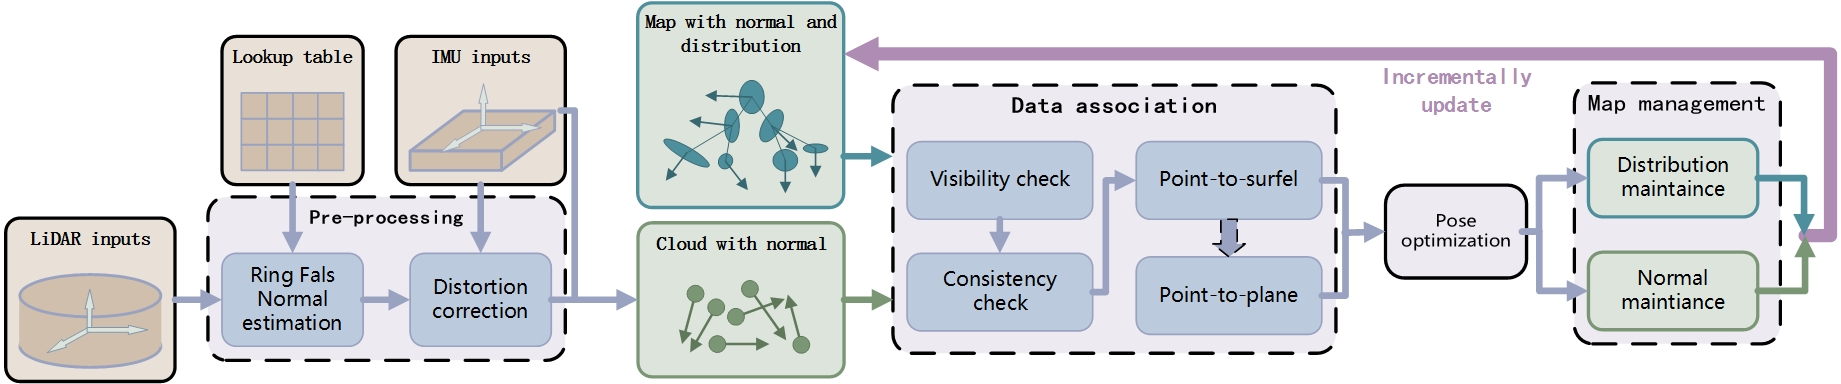
\includegraphics[width=16cm]{fig/overview_3.jpg}
        \caption{System overview of LOG-LIO}
        \label{fig_overview}
\end{figure*}
The pipeline of LOG-LIO receives inputs from a 3D LiDAR and an IMU, as shown in Fig. \ref{fig_overview}.
For a new input scan, we first use Ring FALS to estimate the normal of the raw points.
After correcting distortion with IMU measurements, association is performed between the undistorted point cloud and the map according to their local geometric information.
We integrate the measurements of IMU and optimize the poses of the body via iEKF, like FAST-LIO.
After optimization, new points are added to the map managed by the extended ikd-tree, and the distribution within the voxel is incrementally maintained to ensure its accuracy while considering the normals, and fixed after convergence.

Our system takes IMU frame as the body frame, where system state $\mathbf{x}$ can be written as:
\begin{equation}
        \mathbf{x} = \left[^\mathcal{W}\mathbf{R}^T_\mathcal{I}\ ^\mathcal{W}\mathbf{p}^T_\mathcal{I}\ ^\mathcal{W}\mathbf{v}^T_\mathcal{I}\ \mathbf{b}^T_\omega\ \mathbf{b}^T_a\ ^\mathcal{W}\mathbf{g}^T\right]
        \label{eq_x}
\end{equation}
where$^\mathcal{W}\mathbf{R}^T_\mathcal{I}$, $^\mathcal{W}\mathbf{p}^T_\mathcal{I}$ and $^\mathcal{W}\mathbf{v}^T_\mathcal{I}$ are the attitude, position and velocity of IMU in the world frame (i.e., the first IMU frame), $\mathbf{b}^T_\omega$ and $\mathbf{b}^T_a$ are gyroscope and accelerometer bias respectively, $^\mathcal{W}\mathbf{g}^T$ is the known gravity vector in the world frame.

\section{Ring FALS Normal Estimator}
\label{sec:ring_fals}
For a LiDAR-based SLAM system, searching the neighborhood with the assistance of the KDtree and performing eigen analysis on the matrix $\boldsymbol{M}$ in (\ref{eq_M}) are far overloaded.

In this paragraph, we revisit FALS\cite{badino2011fast}.
Removing the scale factor $d$ to eliminate the constraint on normal gives:
\begin{equation}
        \widetilde{e} = \sum_{i = 1}^{n}(\boldsymbol{p}_i^T \widetilde{\boldsymbol{n}} - 1)^2
        \label{eq_pn_1}
\end{equation}
where $ \widetilde{\boldsymbol{n}}$ is defined up to a scale factor.
By reformulating (\ref{eq_pn_1}), the following is obtained:
\begin{equation}
        \widetilde{e} = \sum_{i = 1}^{n}r_i^2(\boldsymbol{v}_i^T \widetilde{\boldsymbol{n}} - r_i^{-1})^2
        \label{eq_rvn_r}
\end{equation}
where $r_i$ is the range and $\boldsymbol{v}_i$ implies the bearing information of the target points related to LiDAR.
Thanks to the high-resolution LiDAR, it can be assumed that the range of points within a small region are similar.
Removing $r_i^2$ from (\ref{eq_rvn_r}) to obtain an approximation:
\begin{equation}
        \widehat{e} = \sum_{i = 1}^{n}(\boldsymbol{v}_i^T \widehat{\boldsymbol{n}} - r_i^{-1})^2
        \label{eq_vn_r}
\end{equation}
the normal $\widehat{\boldsymbol{n}}$ with the closed form solution $\widehat{\boldsymbol{n}} = \widehat{\boldsymbol{M}}^{-1}\widehat{\boldsymbol{b}}$ where $\widehat{\boldsymbol{M}} =  \sum_{i = 1}^{n}\boldsymbol{v}_i\boldsymbol{v}_i^T$ and $\widehat{\boldsymbol{b}} = \sum_{i = 1}^{n}\boldsymbol{v}_i/r_i$.
The box-filtering techniques\cite{mcdonnell1981box} are available to minimize the number of operations to compute the vector $\widehat{\boldsymbol{b}}$ and the matrix $\widehat{\boldsymbol{M}}^{-1}$.
Furthermore, the matrix $\widehat{\boldsymbol{M}}^{-1}$ depends only on the constant structural information $\boldsymbol{v}$, independent of the range $\boldsymbol{r}$.
Hence, the matrix $\widehat{\boldsymbol{M}}^{-1}$ can be precomputed as a lookup table for the certain LiDAR.

Obviously, a low-resolution lookup table can further improve the computational efficiency, which is similar to downsampling.
But in this work, we employ the Ring FALS to all new scan points for obtaining dense normals.
Flipping the normals toward LiDAR and then applying image blurring techniques to smooth the normals can further improve the consistency of the local geometric information.

Notably, in the association module of LOAM, a point finds its $k$ nearest points by traversing adjacent scanning lines, but this is still a time-consuming step.
By pre-computing the lookup table, normal estimation avoids the slow searching process.
% \begin{equation}
%         \begin{array}{c} 
%         row\_i = ring(\boldsymbol{p}_i) \\
%         column\_i = \theta_i / res \\
%         \end{array}
%         \label{eq_r_ij}
% \end{equation}
% with horizon angle resolution $res$.

\section{Points Distribution Estimation}
\label{sec:distribution_estimation}
The widely used maps in SLAM systems record only the coordinates of points, and the sparsity of map points results in inaccurate representation of the environment, which may provide incorrect constraints and ultimately reduce the accuracy of pose estimation.
To build a high-quality map, we incrementally maintain the points distribution within each voxel.

The distribution of points within a voxel can be represented by the covariance matrix $\boldsymbol{M}$ in (\ref{eq_M}), which can be simplified as:
\begin{equation}
        \boldsymbol{M} = \mathcal{S}_n - \frac{1}{n} \mathcal{P}_n \mathcal{P}_n^T
        \label{eq_M_simp}
\end{equation}
where $\mathcal{S}_n $ denotes $\sum_{i = 1}^{n}\boldsymbol{p}_i \boldsymbol{p}_i^T$ and $\mathcal{P}_n$ denotes $\sum_{i = 1}^{n}\boldsymbol{p}_i $.
Due to the symmetric nature of the matrix $\boldsymbol{M}$, only the six elements in its upper right corner need to be recorded in the computation.
Two distributions with $n$ and $m$ points, respectively, are merged as follows:
\begin{equation}
        \boldsymbol{M}' = \mathcal{S}_n + \mathcal{S}_m - \frac{1}{n + m}(\mathcal{P}_n + \mathcal{P}_m)(\mathcal{P}_n + \mathcal{P}_m)^T
        \label{eq_M_merge}
\end{equation}
% where $m = 1$ means that a new point is added to the voxel that already has $n$ points, and its distribution is updated incrementally.
For a single point is added to the voxel that already has $n$ points, one can ues (\ref{eq_M_merge}) and set $m$ to 1.

The accurate representation of a distribution requires a large number of points.
For a newly created voxel, only its $\mathcal{S}$, $\mathcal{P}$ and the number of points need to be updated incrementally.
% We compute the distribution after the points of a voxel reach a certain number $\eta$ (we use $\eta = 40$).
Because of the limited FoV, for a high-quality map, point cloud should be collected from multiple places, which is historical and accumulated gradually.
Tuning the size of downsampling in pre-processing limits the number of points added to each voxel, thus balancing computational efficiency and accuracy.
% We set the downsampling grid in data pre-processing to have the same size as the map to ensure that at most one point falls within one voxel at a time, because it has already filtered out representative points for us.
% To balance efficiency and accuracy, we fix the distribution of voxels after the inside points reaches $2\eta$.
%merge normal distribution
% To incorporate the current and historical local geometric information in this work, \ie{the normal from Ring FALS and point distribution of corresponding voxel},
% we also perform mean filtering on the historical normals, denoted as $\boldsymbol{n}_r$.
% As long as the angle between the direction of $\boldsymbol{n}_r$ and $\boldsymbol{n}_d$ converge, \ie{the angle is less than 20 degree}, we consider that the distribution tends to stabilize and the normal of the voxel is fixed as the mean value of $\boldsymbol{n}_r$ and $\boldsymbol{n}_d$.
As long as the directions of $\boldsymbol{n}_r$ (introduced in \ref{sec:data_pre}) and $\boldsymbol{n}_d$ converge, we consider that the distribution stabilizes and fix it.

\section{System Description}
\label{sec:system_description}

\subsection{Data Pre-processing}
\label{sec:data_pre}
To profile the environment with accurate local geometric information, instead of performing feature extraction on the raw points as in LOAM, LOG-LIO directly use Ring FALS (see \ref{sec:ring_fals} for details) to estimate the normal of each point, denoted as $\boldsymbol{n}_r$.
Subsequently, voxel grid downsampling and backward propagation based on IMU measurements are used for point reduction and distortion correction, respectively.
% In addition to the 3D coordinates of the points, all methods we used also consider normals.

\subsection{Data Association}
\label{sec:data_association}
The IMU measurements are integrated from the previous frame as a prediction of the pose $\widehat{\mathbf{x}}_{k}$ at the beginning of data association.
With the prediction, each new coming LiDAR point $^\mathcal{L}\boldsymbol{p}_i$ transforms  the world frame $^\mathcal{W}\boldsymbol{p}_i = ^\mathcal{W}\widehat{\boldsymbol{T}}_\mathcal{I}\  ^\mathcal{I}\boldsymbol{T}_\mathcal{L}\  ^\mathcal{L}\boldsymbol{p}_i$.

Having normal and distribution of map points, LOG-LIO perform high-quality data association as follows:
\subsubsection{Visibility and Consistency Checks}
Map points are not visible to the LiDAR if the angle between the normal of the map point and the ray (vector from the query point to the LiDAR) is greater than 90 degrees.
This false association usually occurs indoors, where the two planes of an object (e.g., a wall) are close to each other, which is called the double-side issue\cite{zhou2021lidar}.
This incorrect association is eliminated directly.

The average angle between the normal of the query point and the normals of the associated map points indicates consistency.
If the average angle is larger than $\alpha$ ($\alpha = 60^\circ$ in this paper), we consider it an inconsistent association and discard it.

\subsubsection{Hierarchical Association}
% \begin{figure}[!ht]
%         \centering
%         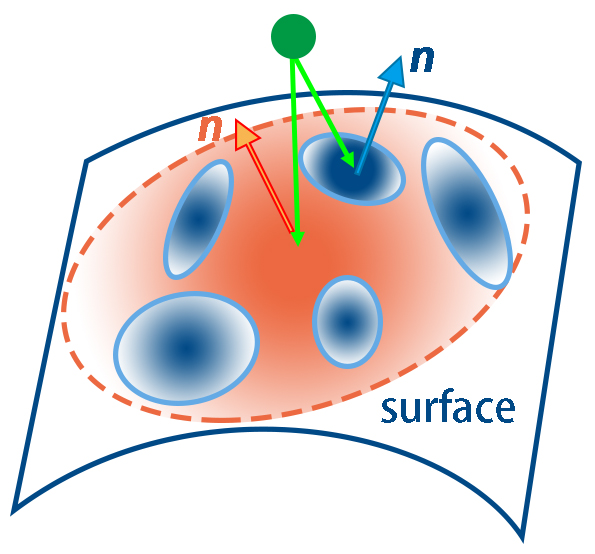
\includegraphics[width=3.5cm]{fig/data_association_2.jpg}
%         \caption{Illustration of the hierarchical data association.
%                 The green point is the query point, and the blue ellipses represent its 5 nearest neighbors in the extended ikd-tree.
%                 We first merge the 5 blue nodes into  the large-scale orange surfel for association.
%                 If the large-scale association is not satisfied, we associate the query point to the small-scale surfel of the nearest node.}
%         \label{fig_association}
% \end{figure}
%voxels large surfel -> point surfel -> plane
For query points satisfy visibility and consistency checks,
a robust and accurate hierarchical association with point-to-surfel priority over point-to-plane and large-scale over small-scale is performed.
% we compute the residual of the query point with the associated map points.
% We design a scheme for calculating residuals, where the priority of surfel is higher than plane and the large-scale over the small-scale.

Modeled by distributions, the surfel represents more accurate local geometric information than coordinates.
Large-scale surfel can be approximated by merging multiple small-scale distributions (see \ref{sec:surfel} for details) and is insensitive to noise thus providing more robust constraints than small-scale surfel.
The point-to-surfel distance implies the quality of the constraint.
For constraints with low-quality large-scale surfel, we associate the query point with the surfel of the voxel where the point is located, which must already be fixed.

% For large-scale surfel residuals, we first merge the distribution of the fixed map voxels where the $k$ associated map points are located according to (\ref{eq_M_merge}), as shown in Fig. \ref{fig_association}.
% Then compute the point-to-surfel distance, which is the distance from the query point to $\mathcal{P}/n$(the mean of the distribution) along the direction of $\boldsymbol{n}_d$ (eigenvector corresponding to the smallest eigenvalue) of the merged distribution.
% If the distance greater than $d_1$ (we use $d_1 = 0.15$), we consider it a large-scale surfel association of poor quality and do not adopt it.

% For small-scale surfel residuals, it is first necessary to satisfy that the query point and the nearest point are located in the same fixed map voxel.
% The point-to-surfel distance is computed in the same way with above.
If the quality of all surfel is poor, LOG-LIO follows LOAM for point-to-plane association.
% If the above two association with surfel cannot be satisfied, we compute the point-to-plane distance as LOAM.

\subsection{Pose optimization}
\label{sec:pose_optimization}

%iEKF
%prediction
We adopt the iterated Kalman filter from FAST-LIO2 to optimize the pose.
The prediction step of the Kalman filter implemented by integrating the IMU measurements from the last optimized state $\overline{\mathbf{x}}_{k-1}$ with the covariance matrix $\overline{\mathbf{P}}_{k-1}$.

%residual
% For residuals computation, we compute the distances satisfying the point-to-surfel and point-to-plane associations respectively.
For a point $^\mathcal{W}\boldsymbol{p}_i$ is already transformed to the world frame, the residual $z_i$ is computed as:
\begin{equation}
        \mathbf{z}_i = \boldsymbol{n}_j(^\mathcal{W}\boldsymbol{p}_i - ^\mathcal{W}\boldsymbol{q}_j)
        \label{eq_z_i}
\end{equation}
where $\boldsymbol{n}_j$ is the normalized normal of the associated surfel or plane of $\boldsymbol{p}_i$, and $^\mathcal{W}\boldsymbol{q}_j$ is the point lying on the corresponding element.

%update
Denote $\widehat{\mathbf{x}}_{k}$ and $\widehat{\mathbf{P}}_{k}$ with propagated state and covariance respectively, and they represent the prior Gaussian distribution for the state.
Incorporate the prior distribution with all point-to-surfel and point-to-plane measurement models from (\ref{eq_z_i}) yields the maximum a-posterior estimate(MAP):
\begin{equation}
        \begin{aligned}
                \underset{\widetilde{\mathbf{x}}_k^\kappa}{min} & ( \|\mathbf{x}_{k}\boxminus \widehat{\mathbf{x}}_k\Vert^2_{\widehat{\mathbf{P}}_k}                                     \\
                                                                & +\sum_{i\in surfel} \|\mathbf{z}_i^\kappa + \mathbf{H}_i^\kappa \widetilde{\mathbf{x}}_k^\kappa \Vert_{\mathbf{R}_i}^2 \\
                                                                & +\sum_{j\in plane} \|\mathbf{z}_j^\kappa + \mathbf{H}_j^\kappa \widetilde{\mathbf{x}}_k^\kappa \Vert_{\mathbf{Q}_j}^2)
        \end{aligned}
        \label{eq_map}
\end{equation}
where $\widetilde{\mathbf{x}}_k^\kappa$ is the error of the $\kappa$-th iterate update at time $k$, $\mathbf{H}_i^\kappa$ and $\mathbf{H}_j^\kappa$ are Jacobian matrices with respect to $\widetilde{\mathbf{x}}_k^\kappa$, $\mathbf{R}_i$ and $\mathbf{Q}_j$ come from the raw measurement noise.
The Kalman gain can be computed in an efficient way that the computation load depends on the state dimension instead of the measurement dimension.
Due to limited space, we refer readers to \cite{xu2021fast,xu2022fast} for details.
%todo figure

\subsection{Map Management}
\label{sec:map_management}
LOG-LIO manages maps with voxels.
However recalculating the voxel point distribution when adding new points is overburdening for the LIO system.
To incrementally maintain the points distribution within each voxel, we extend the ikdtree and mapping each voxel to a corresponding node.

% %fix distribution
% % The point distribution within the voxel represents its local geometric information, which should be historical and gradually accumulated.
% % This coincides with the fact that the accurate representation of point distribution requires a large number of points.

% %merge normal distribution
% To incorporate the current and historical local geometric information in this work, \ie{the normal from Ring FALS and point distribution of corresponding voxel},
% we also perform mean filtering on the historical normals, denoted as $\boldsymbol{n}_r$.
% As long as the angle between the direction of $\boldsymbol{n}_r$ and $\boldsymbol{n}_d$ converge, \ie{the angle is less than 20 degree}, we consider that the distribution tends to stabilize and the normal of the voxel is fixed as the mean value of $\boldsymbol{n}_r$ and $\boldsymbol{n}_d$.


\section{EXPERIMENTAL RESULTS}
\label{sec:experimental_results}

\subsection{Implementation}
For the Ring FALS normal estimator, the lookup table is pre-built following $\mathcal{V}(ring\_i,\ column\_i) = \overline{\boldsymbol{v}}_i$, where $row\_i = ring(\boldsymbol{p}_i)$, $column\_i = \theta_i / res$ and $res$ is the preset horizontal angle resolution.
For each node of the extended ikdtree, we incrementally maintain the points distribution after the number of points in the voxel has accumulated to a certain number $\eta$ ($\eta=25$ in this paper).
To balance efficiency and accuracy, we fix the distribution of voxels after the inside points reach $2\eta$.
The downsampling grid in data pre-processing is set to have the same size as the map to ensure that at most one point falls within a voxel for each frame.
As long as the angle between the direction of $\boldsymbol{n}_r$ and $\boldsymbol{n}_d$ is less than 20 degree, the distribution is considered to be stabilized and the normals of the voxels are fixed as the average of $\boldsymbol{n}_r$ and $\boldsymbol{n}_d$.

\subsection{Experimental Design}
The experiment focuses on the following two key points:
\begin{itemize}
        \item
              Ring FALS estimates the normal of LiDAR points in real-time and accurately represents environmental information.
        \item
              By incorporating normal and points distribution estimation to accurately represent local geometric information, LOG-LIO improves the accuracy of pose estimation.
\end{itemize}

We conduct extensive experiments on the public datasets M2DGR\cite{yin2021m2dgr} and NTU VIRAL\cite{nguyen2022ntu} to prove the above two points.
% In this section, we experimentally demonstrate that accurate local geometric information is crucial for the LIO systems.
% Extensive experiments are conducted on the public datasets M2DGR\cite{yin2021m2dgr} and NTU VIRAL\cite{nguyen2022ntu}.
% The results show that by incorporating normal and point distribution estimation, LOG-LIO is more robust and accurate than other state-of-the-art methods.
Experiments were carried out on a PC with Ubuntu 18.04, equipped with an Intel Core Xeon(R) Gold 6248R 3.00GHz processor and 32G RAM.

% In this section, for the computation efficiency and accuracy of Ring FALS and LOG-LIO proposed in this paper, extensive experiments are conducted on the public datasets M2DGR\cite{yin2021m2dgr} and NTU VIRAL\cite{nguyen2022ntu}.
% We implement the proposed Ring FALS normal estimator and LOG-LIO in C++ and Robot Operating System(ROS).
% By comparing with the PCL\cite{rusu20113d} normal estimation tools, which is a widely used library in point cloud algorithms, we first prove the efficiency and accuracy of Ring FALS.
% Then we combine Ring FALS normal estimator into LOG-LIO to demonstrate the accuracy of the proposed LiDAR-inertial odometry.

\subsection{Ring FALS Normal Estimation}
% In the implementation of PCL normal estimation, it consider that the point cloud is unordered, so a KDtree is built for searching neighborhoods.
% The procedure is similar to traditional least squares.
We compare Ring FALS and PCL\cite{rusu20113d} normal estimation tools.
The implementation of PCL normal estimation is based on traditional least squares with the assistance of KDtree.
By approximating the problem as estimating the normal to a plane tangent to the surface where the point is located, it becomes a least-squares plane fitting estimation problem.
PCL also provides an additional implementation to speed up the computation, which uses the multi-threaded paradigm of OpenMP\cite{chandra2001parallel}.
Considering that normal smoothing of disordered point cloud is another time-consuming process, the results of PCL are not further modified, but only smooth the normals of Ring FALS.

\begin{figure*}[!ht]
        \centering
        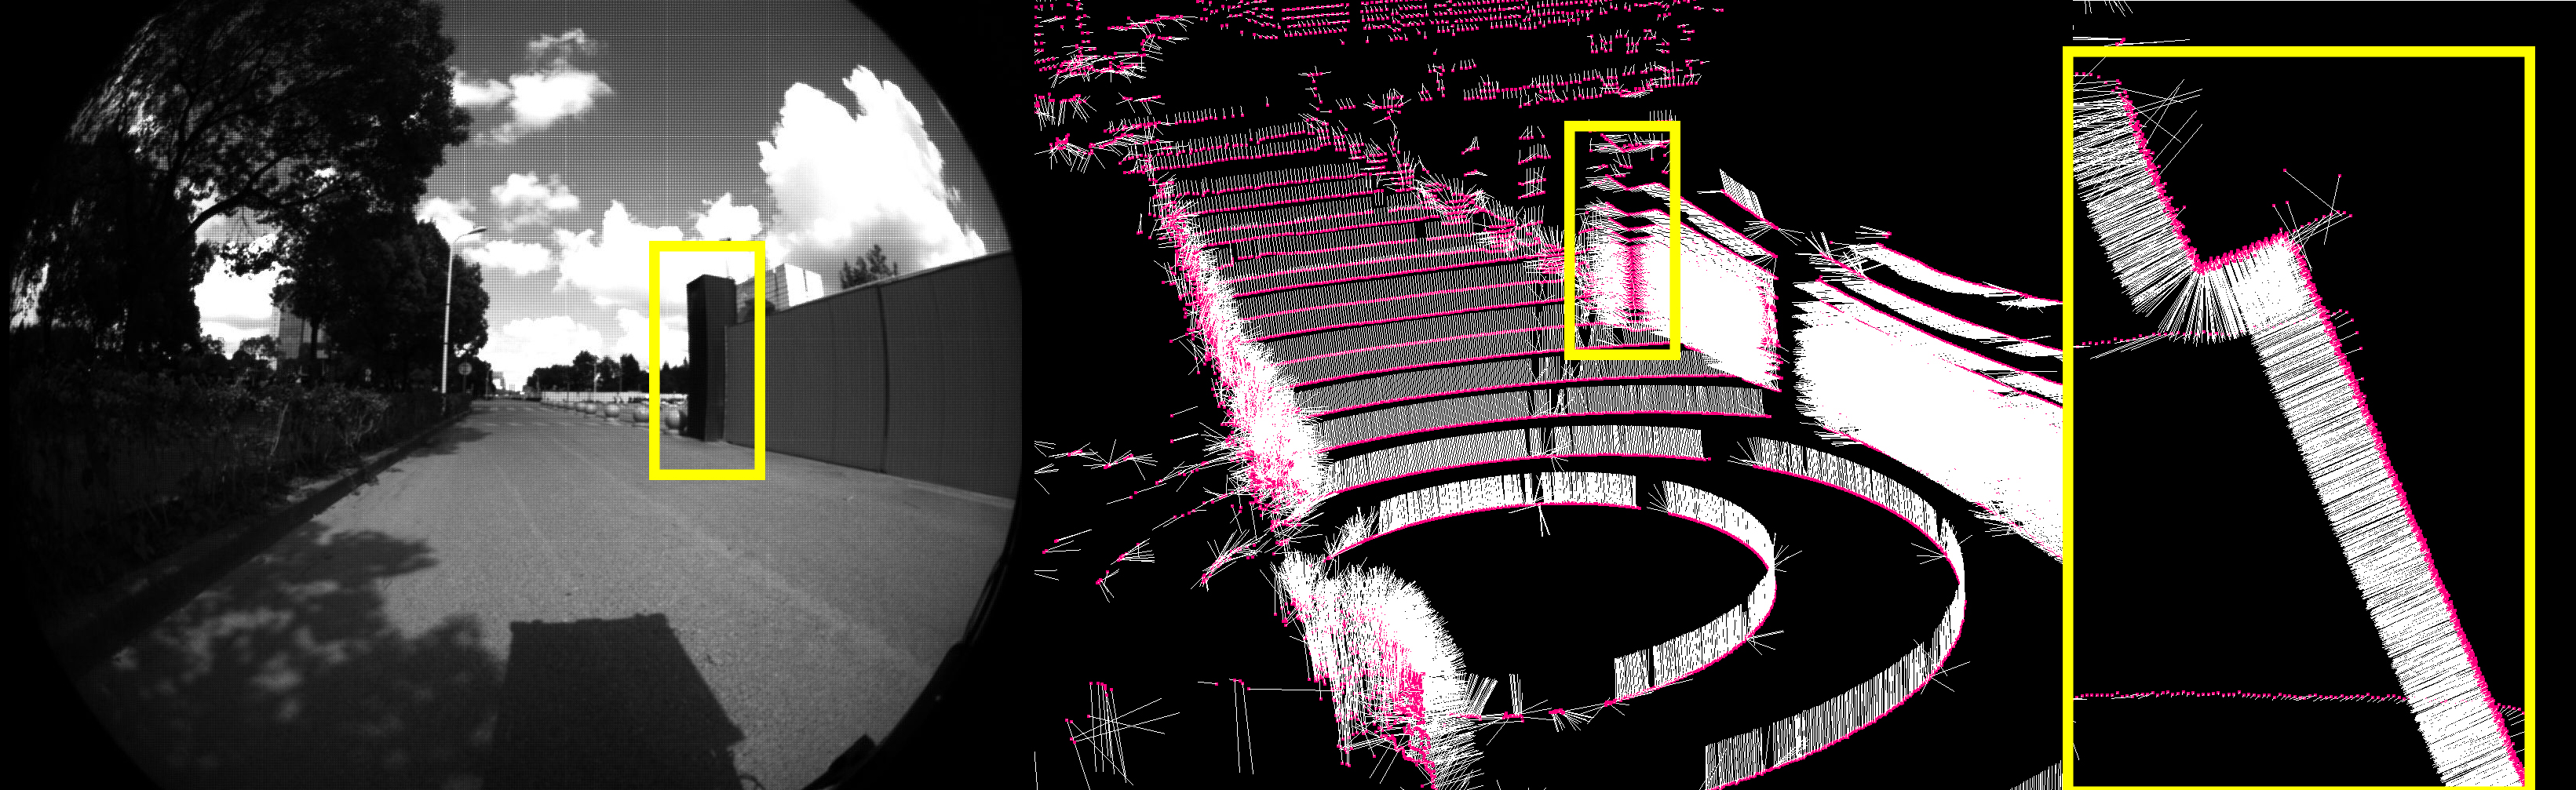
\includegraphics[width=17cm]{fig/normals.jpg}
        \caption{The starting position of the sequence \emph{gate03} of M2DGR dataset.
                The white lines represent normalized normals from Ring FALS estimation.}
        \label{fig_normal}
\end{figure*}
We visualize the normalized normals at the starting position of the sequence \emph{gate03} of the M2DGR dataset to provide a intuitive evaluation.
As shown in Fig. \ref{fig_normal}, almost all ground point normals are vertically upward.
For the pillar shown in the yellow box in Fig. \ref{fig_normal}, from the top view, the normal at each point is perpendicular to the wall and the normal at the corner is smoothly articulated with the two adjacent sides.
For more visualization results of normal estimation, we recommend readers go to \href{https://github.com/tiev-tongji/RingFalsNormal}{https://github.com/tiev-tongji/RingFalsNormal}.

Table \ref{tab_ringfals_time} shows the average normal estimation processing times for a single scan of LiDAR used in the M2DGR and NTU VIRAL datasets, respectively.
For a single scan of about 57,600 points for the Velodyne-32 LiDAR, Ring FALS takes a tenth of the time spent on PCL, and a quarter of it even compared to the OMP version.
For the Ouster-16 LiDAR, the time consumption of Ring FALS is much less than that of PCL, no matter for the single threaded or OMP version.
Analyzing the results of PCL, although Ouster-16 LiDAR has fewer points than Velodyne-32, the consumption time increases instead.
The reason is that one of the most time-consuming parts of the PCL normal estimation is the KDtree neighborhood searching, which is related to the structure of the KDtree.
And the structure of the constructed KDtree depends on the complexity of the environment, hence simply reducing the number of points cannot guarantee the speedup of the normal estimation in PCL.
This means treating the point cloud as disordered, the sparsity of the point cloud could become a computational burden for the normal estimation.
Although multi-threading speeds up the computation, how to choose a reasonable number of threads is also a problem to be considered.
Ring FALS circumvents these problems because the structural information of the LiDAR is implicitly included in the lookup table.
\begin{table*}[htb!]
        \caption{The Mean Running Time(ms) of Normal Estimation for A Single Scan to Certain LiDARs}
        \centering
        \begin{tabular}{c|c|c c c|c|c|c}
                \toprule
                            & \multirow{2}{*}{points} & \multicolumn{4}{c|}{Ring FALS} & \multicolumn{2}{c}{PCL}                                                               \\
                            &                         & projection                     & box-filtering           & smoothing & total          & single thread & OMP 10 threads \\
                \midrule
                Velodyne-32 & 57600                   & 2.045                          & 2.540                   & 3.199     & \textbf{7.784} & 79.811        & 26.355         \\
                Ouster-16   & 16384                   & 0.560                          & 1.221                   & 0.815     & \textbf{2.597} & 155.972       & 39.664         \\
                \bottomrule
        \end{tabular}
        \label{tab_ringfals_time}
\end{table*}

\subsection{Odometry Accuracy Evaluation}
% We conduct experiments using the public dataset M2DGR and NTU VIRAL to evaluate the performance of the proposed LOG-LIO and compare our methods with two state-of-the-art LiDAR-Inertial SLAM methods, namely LIO-SAM\cite{shan2020lio} and FAST-LIO2\cite{xu2022fast}.
We compare LOG-LIO with two state-of-the-art LiDAR-Inertial SLAM methods, LIO-SAM\cite{shan2020lio} and FAST-LIO2\cite{xu2022fast}.
LOG-LIO and FAST-LIO2 estimate odometry without loop closure, for a fair comparison we disable the loop closure of LIO-SAM.
Source code for LIO-SAM and FAST-LIO2 are obtained from the addresses they provide, and parameters remain as defaults.
The root-mean-square error(RMSE) of the absolute trajectory error (ATE) is adopted to assess the accuracy of poses.

\subsubsection{M2DGR Datasets}
The dataset is collected by a ground robot and captured in diverse scenarios including both indoor and outdoor environments.
The ground truth trajectories were obtained by a laser 3D tracker, motion capture device and an RTK receiver.
% We use the Velodyne VLP-32C LiDAR and Handsfree A9 IMU in the dataset to test the performance of LIO-SAM, FAST-LIO2 and LOG-LIO.
% For the data collected indoor, the robot moves in a hall in the \emph{hall} sequences, and the robot moves from outdoor to indoor though a door in the \emph{door} sequences.
% The \emph{gate}, \emph{walk} and \emph{street} sequences collected data outdoors.
In all experiments, the resolution of maps and new scan downsampling size was set to 0.4 m to reduce the interference of the point cloud density.
Due to the instability of the RTK signal, the first 100 seconds and the last 100 seconds of \emph{street07} and \emph{street10} are discarded in the experiment, respectively.
We evaluate the method combining the proposed Ring FALS, visibility and consistency checks (denoted as LOG-C) as ablation experiments.

Table \ref{tab_m2dgr} reports the result of our experiments.
It can be seen that the trajectory accuracy of LOG, LOG-C and FAST-LIO2 is close in indoor scenes and outperforms LIO-SAM in most sequences.
This makes sense because the number of plane features has a quantitative advantage in indoor scenes, where neighborhood map points generally form true planes.
Therefore, the point-to-plane data association provides good constraints for pose estimation.
Conversely, as errors accumulate, the point-to-line data association of LIO-SAM may provide negative effects.
For outdoors, map points are relatively sparse compared to indoors, especially for the \emph{street} sequences, where the robot moves on empty urban roads at night.
Fig. \ref{fig_street10} shows the trajectories of the sequence \emph{street10} for qualitative comparison.
The outstanding performance of LOG proves that surfel associated with map voxels better represents local geometric information in scenes with sparse points.
% The point-to-surfel data association with visibility and consistency checks are preferable, so LOG-LIO performs better.
However, the point-to-line and point-to-plane data associations become unstable as can be seen from the performance of LIO-SAM.
Overall, with the visibility and consistency checks, LOG-C slightly improves the average accuracy.
Combined with our proposed hierarchical data association and map management schemas, LOG performs the best, achieving the minimum error in 13 of the 21 sequences presented.
\begin{figure*}[!ht]
        \centering
        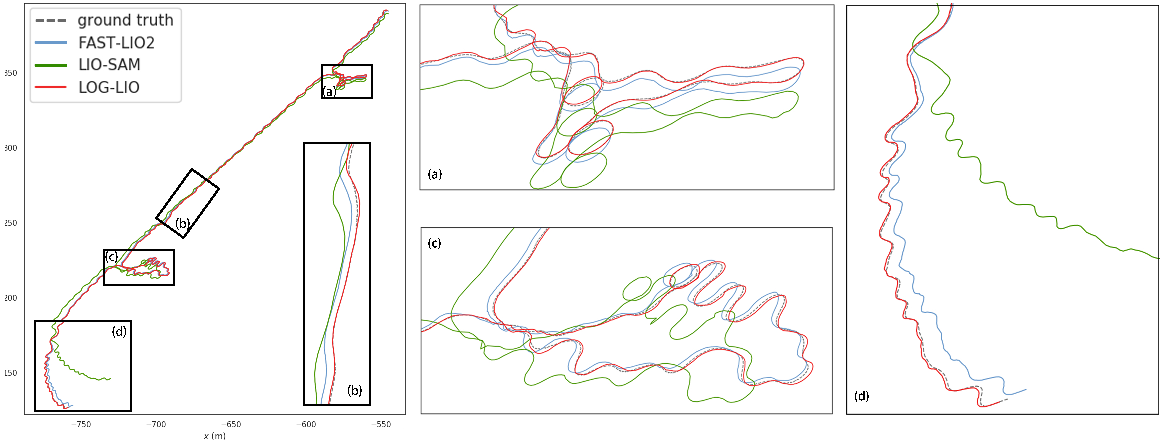
\includegraphics[width=16cm]{fig/street10.pdf}
        \caption{Localization estimates in sequence \emph{street10} of the M2DGR dataset.
                 The zoomed in image of the colored boxes corresponds to the boxes of the same color in the trajectory.}
        \label{fig_street10}
\end{figure*}
%excel to latex tool: https://www.tablesgenerator.com/
\begin{table}[htb!]
        \caption{The Translation RMSE(m) Results of Pose Estimation Comparison on the M2DGR Dataset}
        \centering
        \begin{tabular}{c|c|c|c|c|c}
                \toprule
                \multirow{2}{*}{Seq} & duration & \multirow{2}{*}{LOG} & \multirow{2}{*}{LOG-C} & \multirow{2}{*}{LIO-SAM} & \multirow{2}{*}{FAST-LIO2} \\
                                     & (s)      &                      &                        &                          &                            \\
                \midrule
                gate01               & 172      & 0.137                & \textbf{0.133}         & 0.170                    & 0.134                      \\
                gate02               & 327      & \textbf{0.290}       & 0.304                  & 0.318                    & 0.304                      \\
                gate03               & 283      & \textbf{0.108}       & \textbf{0.108}         & 0.110                    & 0.110                      \\
                walk01               & 291      & 0.079                & 0.082                  & \textbf{0.078}           & 0.091                      \\
                door01               & 461      & \textbf{0.250}       & \textbf{0.250}         & 0.271                    & 0.253                      \\
                door02               & 127      & \textbf{0.178}       & \textbf{0.178}         & 0.185                    & \textbf{0.178}             \\
                street01             & 1028     & \textbf{0.212}       & \textbf{0.212}         & 0.586                    & 0.221                      \\
                street02             & 1227     & 2.537                & \textbf{2.315}         & 3.619                    & 2.394                      \\
                street03             & 354      & \textbf{0.140}       & 0.146                  & 0.149                    & \textbf{0.140}             \\
                street04             & 858      & \textbf{0.525}       & 0.591                  & 1.022                    & 0.568                      \\
                street05             & 469      & 0.342                & \textbf{0.310}         & 0.491                    & 0.319                      \\
                street06             & 494      & 0.392                & 0.437                  & \textbf{0.373}           & 0.439                      \\
                street07             & 829      & 2.301                & 3.468                  & \textbf{1.514}           & 3.422                      \\
                street08             & 491      & \textbf{0.169}       & 0.179                  & 0.212                    & 0.182                      \\
                street09             & 907      & 3.010                & 3.570                  & \textbf{2.447}           & 3.613                      \\
                street10             & 810      & \textbf{0.329}       & 1.213                  & 8.097                    & 1.256                      \\
                hall01               & 351      & \textbf{0.256}       & 0.257                  & 0.287                    & 0.257                      \\
                hall02               & 128      & \textbf{0.275}       & \textbf{0.275}         & 0.290                    & 0.279                      \\
                hall03               & 164      & \textbf{0.340}       & 0.343                  & 0.612                    & 0.346                      \\
                hall04               & 181      & \textbf{0.943}       & \textbf{0.943}         & 1.078                    & 0.945                      \\
                hall05               & 402      & 1.047                & \textbf{1.046}         & 1.010                    & \textbf{1.046}             \\
                \midrule
                mean                 &          & \textbf{0.660}       & 0.779                  & 1.091                    & 0.786                      \\
                \bottomrule
        \end{tabular}
        \label{tab_m2dgr}
\end{table}
% \COMMENT{hk: fig of map normals, double-side issue}

\subsubsection{NTU VIRAL Datasets}
NTU VIRAL performs data collection on an Unmanned Aerial Vehicle (UAV) platform with ground truth obtained by a laser-tracker total station with centimeter-level accuracy.
The horizontal Ouster 16-channel OS1 LiDAR and VectorNav VN100 IMU are used for the experiments in this paper.
% The environments consist of indoor and outdoor spaces within a volume of 50 m radius.
Compared with M2DGR, the LiDAR used by VIRAL has a sparser point cloud, making it more challenging to estimate poses in open areas.
In all experiments, the resolution of maps and new scan downsampling size is set to 0.5 m.

% Table \ref{tab_viral} shows the comparison study for LOG-LIO against the state-of-the-art methods LIO-SAM and FAST-LIO2.
As shown in Table \ref{tab_viral}, LOG-LIO gives the best results in most experiments, followed closely by FAST-LIO2, while LIO-SAM fails more often due to the sparsity of LiDAR point cloud and map.
As the sequences \emph{nya} and \emph{tnp} traverse in small indoor areas, the errors of LOG-LIO and FAST-LIO2 are close, which is similar to M2DGR.
For the sequences \emph{eee}, \emph{sbs} and \emph{rtp}, although they are outdoor scenes, the drone is surrounded by buildings like indoors.
The trajectories of LOG-LIO and FAST-LIO2 are also very close because of the well constrained plane.
However, in the \emph{spms} sequences, the UAV takes off from an area surrounded by buildings and then hovers at an altitude higher than the top of the surrounding buildings.
The sparse point cloud obtained by the horizontal LiDAR has a low overlap with the map, therefore the registration error based on point-to-plane data association is prone to be large.
For LOG-LIO, the points are first associated with the voxels where they are located, and the results show that the proposed hierarchical association tend to be higher-quality constrain.
\begin{table}[htb!]
        \caption{The Translation RMSE(m) Results of Pose Estimation Comparison on the NTU VIRAL Dataset}
        \centering
        \begin{tabular}{c|c|c|c|c}
                \toprule
                % Seq                  & LOG-LIO           & FAST-LIO2             & LIO-SAM                                               \\
                \multirow{2}{*}{Seq} & duration & \multirow{2}{*}{LOG-LIO} & \multirow{2}{*}{FAST-LIO2} & \multirow{2}{*}{LIO-SAM} \\
                                     & (s)      &                          &                            &                          \\

                \midrule
                eee\_01              & 399      & \textbf{0.191}           & 0.193                      & 0.206                    \\
                eee\_02              & 321      & \textbf{0.141}           & 0.142                      & 0.145                    \\
                eee\_03              & 181      & 0.186                    & \textbf{0.185}             & 0.206                    \\
                nya\_01              & 396      & 0.208                    & \textbf{0.204}             & 0.278                    \\
                nya\_02              & 428      & 0.212                    & 0.211                      & \textbf{0.204}           \\
                nya\_03              & 411      & \textbf{0.224}           & \textbf{0.224}             & 0.305                    \\
                sbs\_01              & 354      & \textbf{0.222}           & \textbf{0.222}             & x                        \\
                sbs\_02              & 373      & \textbf{0.208}           & \textbf{0.208}             & 0.211                    \\
                sbs\_03              & 389      & 0.195                    & \textbf{0.194}             & 0.203                    \\
                rtp\_01              & 482      & \textbf{0.206}           & 0.236                      & x                        \\
                rtp\_02              & 453      & 0.201                    & 0.201                      & \textbf{0.182}           \\
                rtp\_03              & 355      & 0.195                    & 0.196                      & \textbf{0.158}           \\
                tnp\_01              & 583      & 0.174                    & \textbf{0.171}             & x                        \\
                tnp\_02              & 457      & \textbf{0.167}           & \textbf{0.167}             & x                        \\
                tnp\_03              & 407      & 0.206                    & \textbf{0.202}             & x                        \\
                spms\_01             & 446      & 1.939                    & \textbf{1.935}             & 0.600                    \\
                spms\_02             & 398      & \textbf{2.401}           & 3.388                      & x                        \\
                spms\_03             & 386      & \textbf{0.684}           & 0.760                      & x                        \\
                \midrule
                mean                 &          & \textbf{0.442}           & 0.502                      & x                        \\
                \bottomrule
        \end{tabular}
        \label{tab_viral}
\end{table}

\subsubsection{Processing Time Evaluation}
\begin{table*}[htb!]
        \caption{The Average Time Consumption(ms) of Each Sequence in The Experiments}
        \centering
        \begin{tabular}{c|c|c|c|c|c|c|c|c|c|c|c|c}
                \toprule
                {}        & \multicolumn{5}{c|}{M2DGR} & \multicolumn{6}{c|}{NTU VIRAL} &                                                                                                  \\
                {}        & gate                       & walk                           & door   & street & hall   & eee    & nya    & sbs    & rtp    & tnp    & spms   & mean            \\
                \midrule
                LOG-LIO   & 39.839                     & 40.382                         & 18.073 & 36.380 & 18.603 & 18.806 & 15.421 & 15.724 & 23.530 & 17.122 & 20.948 & 25.321          \\
                FAST-LIO2 & 31.378                     & 32.276                         & 14.754 & 28.970 & 15.509 & 15.705 & 12.476 & 12.785 & 21.006 & 13.340 & 17.106 & \textbf{20.523} \\
                \bottomrule
        \end{tabular}
        \label{tab_lio_time}
\end{table*}
We statistics the average time consumption of LOG-LIO and FAST-LIO2 in every sequence as shown in table \ref{tab_lio_time}.
Since the distribution of points within the map voxels is maintained incrementally, the average processing time on each scan in LOG-LIO is slightly longer than in FAST-LIO2.
According to the number of points and the complexity of the environment, LOG-LIO takes about 5 milliseconds more on average, but still meets the real-time requirements.

\section{CONCLUSION AND FUTURE WORK}
\label{sec:conclusion_and_future_work}
This paper proposes LOG-LIO, an online LiDAR-inertial odometry, which incorporates real-time estimation of normal and points distribution to accurately represent the local geometric information.
An efficient normal estimator for LiDAR point cloud, namely Ring FALS, is also presented, which pre-computes the bearing information and uses only the range information to estimate the normal of points. 
LOG-LIO manages the map with an extended ikd-tree and incrementally maintains the normal and points distribution within the map voxels. 
The hierarchical data association schema provides accurate constraints resulting in more accurate pose estimation. 
LOG-LIO outperforms state-of-the-art LIO systems in our experiments on diverse environments. 

For future work, we plan to incorporate dynamic noise removal and loop closure in LOG-LIO to improve stability in dynamic environments and long-term operation.

\bibliographystyle{IEEEtran}
\bibliography{IEEEabrv, paper}

\end{document}